\documentclass[aspectratio=169,11pt]{beamer}
\usetheme{metropolis}
\usepackage{tikz}
\usetikzlibrary{arrows.meta,positioning,decorations.pathmorphing,calc,shapes.geometric}
\usepackage{pgfplots}
\pgfplotsset{compat=1.18}
\usepackage{booktabs}
\usepackage{xcolor}

\definecolor{evidence}{HTML}{2196F3}
\definecolor{choice}{HTML}{E91E63}
\definecolor{geometry}{HTML}{4CAF50}
\definecolor{causal}{HTML}{FF9800}
\definecolor{neutral}{HTML}{9E9E9E}
\definecolor{pass}{HTML}{4CAF50}
\definecolor{fail}{HTML}{F44336}
\definecolor{partial}{HTML}{FF9800}

\title{Geometric Structure in Neural Population Codes}
\subtitle{Subspace geometry, causal interventions, and validity in Steinmetz 2019}
\author{Elliott Tower}
\date{2026}
\institute{}

\begin{document}

\maketitle

%% ============================================================
%% SECTION 1: MOTIVATION
%% ============================================================

\begin{frame}{Why geometry?}
\begin{columns}[T]
\begin{column}{0.55\textwidth}
Most neural analysis asks \emph{what} neurons encode. We wanted to ask what \textbf{shape} that encoding takes---and whether the shape is causally meaningful, not just descriptive.

Geometric methods from ML interpretability (CKA, subspace analysis, interchange interventions) have rarely been applied to real neural data with proper validity checks.

\vspace{1em}
\textbf{Key question:} \\
Do neural populations encode task variables in low-dimensional subspaces, and can we prove it causally?
\end{column}
\begin{column}{0.42\textwidth}
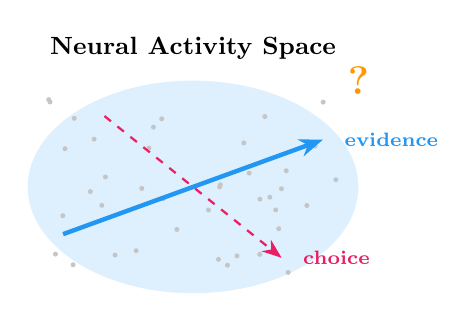
\begin{tikzpicture}[scale=0.75]
  % Neural population cloud
  \fill[evidence!15] (0,0) ellipse (2.8 and 1.8);
  \node[above,font=\small\bfseries] at (0,2.0) {Neural Activity Space};

  % Random dots (neurons/trials)
  \foreach \i in {1,...,40} {
    \pgfmathsetmacro{\rx}{2.5*rand}
    \pgfmathsetmacro{\ry}{1.5*rand}
    \fill[neutral!60] (\rx,\ry) circle (1.2pt);
  }

  % Evidence subspace line
  \draw[evidence,ultra thick,-{Stealth[length=3mm]}] (-2.2,-0.8) -- (2.2,0.8);
  \node[evidence,font=\scriptsize\bfseries,anchor=west] at (2.4,0.8) {evidence};

  % Choice subspace line
  \draw[choice,thick,dashed,-{Stealth[length=2.5mm]}] (-1.5,1.2) -- (1.5,-1.2);
  \node[choice,font=\scriptsize\bfseries,anchor=west] at (1.7,-1.2) {choice};

  % Question mark
  \node[causal,font=\Large\bfseries] at (2.8,1.8) {?};
\end{tikzpicture}
\end{column}
\end{columns}
\end{frame}

%% ============================================================
\begin{frame}{The data: Steinmetz et al.\ 2019}
\begin{columns}[T]
\begin{column}{0.5\textwidth}
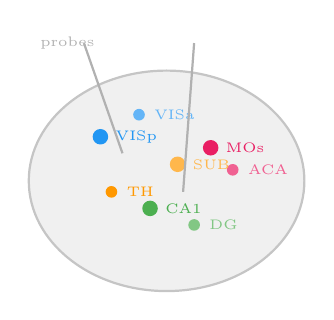
\begin{tikzpicture}[scale=0.7]
  % Mouse head outline (simple)
  \fill[neutral!15] (0,0) ellipse (2.5 and 2);
  \draw[neutral!60,thick] (0,0) ellipse (2.5 and 2);

  % Brain regions as colored dots
  \fill[evidence] (-1.2,0.8) circle (4pt) node[right,font=\tiny,xshift=2pt] {VISp};
  \fill[evidence!70] (-0.5,1.2) circle (3pt) node[right,font=\tiny,xshift=2pt] {VISa};
  \fill[choice] (0.8,0.6) circle (4pt) node[right,font=\tiny,xshift=2pt] {MOs};
  \fill[choice!70] (1.2,0.2) circle (3pt) node[right,font=\tiny,xshift=2pt] {ACA};
  \fill[geometry] (-0.3,-0.5) circle (4pt) node[right,font=\tiny,xshift=2pt] {CA1};
  \fill[geometry!70] (0.5,-0.8) circle (3pt) node[right,font=\tiny,xshift=2pt] {DG};
  \fill[causal] (-1.0,-0.2) circle (3pt) node[right,font=\tiny,xshift=2pt] {TH};
  \fill[causal!70] (0.2,0.3) circle (4pt) node[right,font=\tiny,xshift=2pt] {SUB};

  % Neuropixels probes
  \draw[neutral!80,thick] (-1.5,2.5) -- (-0.8,0.5);
  \draw[neutral!80,thick] (0.5,2.5) -- (0.3,-0.2);
  \node[font=\tiny,neutral!80] at (-1.8,2.5) {probes};
\end{tikzpicture}
\end{column}
\begin{column}{0.5\textwidth}
\begin{itemize}
  \item 39 sessions, 10 mice
  \item \textbf{73 brain regions} recorded simultaneously
  \item Neuropixels probes (high density)
  \item Visual discrimination task \\
    {\small (which side has higher contrast?)}
  \item Trial variables: stimulus evidence, choice, reaction time, feedback
\end{itemize}
\vspace{0.5em}
{\small \textcolor{neutral}{Steinmetz et al., Nature 2019}}
\end{column}
\end{columns}
\end{frame}

%% ============================================================
%% SECTION 2: WHAT WE FOUND
%% ============================================================
\section{What geometry looks like}

%% --- Finding 1: Anti-correlation ---
\begin{frame}{Linear and nonlinear geometry are anti-correlated}
\begin{columns}[T]
\begin{column}{0.5\textwidth}
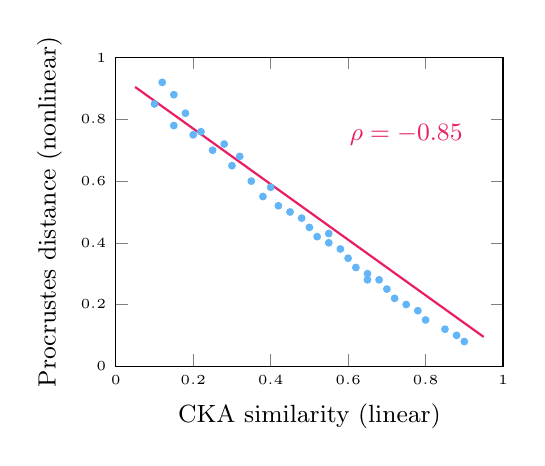
\begin{tikzpicture}
\begin{axis}[
  width=6.5cm, height=5.5cm,
  xlabel={CKA similarity (linear)},
  ylabel={Procrustes distance (nonlinear)},
  xlabel style={font=\small},
  ylabel style={font=\small},
  tick label style={font=\tiny},
  xmin=0, xmax=1, ymin=0, ymax=1,
]
  % Anti-correlated cloud
  \addplot[only marks, mark=*, mark size=1.2pt, evidence!70]
    coordinates {
      (0.1,0.85)(0.15,0.78)(0.12,0.92)(0.2,0.75)(0.18,0.82)
      (0.25,0.7)(0.22,0.76)(0.3,0.65)(0.28,0.72)(0.35,0.6)
      (0.32,0.68)(0.38,0.55)(0.4,0.58)(0.42,0.52)(0.45,0.5)
      (0.48,0.48)(0.5,0.45)(0.52,0.42)(0.55,0.4)(0.58,0.38)
      (0.6,0.35)(0.62,0.32)(0.65,0.3)(0.68,0.28)(0.7,0.25)
      (0.72,0.22)(0.75,0.2)(0.78,0.18)(0.8,0.15)(0.85,0.12)
      (0.88,0.1)(0.9,0.08)(0.15,0.88)(0.55,0.43)(0.65,0.28)
    };
  % Trend line
  \addplot[choice, thick, domain=0.05:0.95] {0.95 - 0.9*x};
  \node[font=\small\bfseries,choice] at (axis cs:0.75,0.75) {$\rho = -0.85$};
\end{axis}
\end{tikzpicture}
\end{column}
\begin{column}{0.48\textwidth}
Regions that look similar in linear geometry look \emph{different} in nonlinear geometry, and vice versa. This was not expected---most prior work treats these as interchangeable.

\vspace{1em}
\textbf{Implication:} \\
You cannot characterize neural geometry with a single metric family. The choice of tool determines what you find.

\vspace{1em}
{\small \textcolor{pass}{\textbf{Validated:}} Held 5 $\to$ 39 sessions; $p \approx 0$}
\end{column}
\end{columns}
\end{frame}

%% --- Finding 2: Spectral universality ---
\begin{frame}{Eigenvalue shapes are universal; trial content is not}
\begin{columns}[T]
\begin{column}{0.5\textwidth}
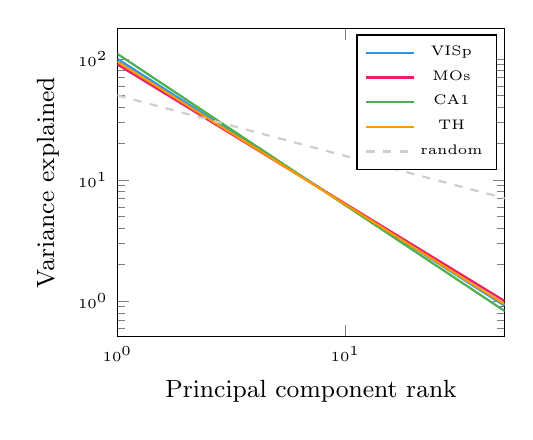
\begin{tikzpicture}
\begin{axis}[
  width=6.5cm, height=5.5cm,
  xlabel={Principal component rank},
  ylabel={Variance explained},
  xlabel style={font=\small},
  ylabel style={font=\small},
  tick label style={font=\tiny},
  xmode=log, ymode=log,
  xmin=1, xmax=50,
  legend style={font=\tiny, at={(0.98,0.98)}, anchor=north east},
]
  % Multiple regions with similar power laws
  \addplot[evidence, thick, domain=1:50, samples=30] {100*x^(-1.2)};
  \addplot[choice, thick, domain=1:50, samples=30] {90*x^(-1.15)};
  \addplot[geometry, thick, domain=1:50, samples=30] {110*x^(-1.25)};
  \addplot[causal, thick, domain=1:50, samples=30] {95*x^(-1.18)};
  \addplot[neutral!50, thick, dashed, domain=1:50, samples=30] {50*x^(-0.5)};
  \legend{VISp, MOs, CA1, TH, random}
\end{axis}
\end{tikzpicture}
\end{column}
\begin{column}{0.48\textwidth}
\textbf{Universal:} eigenvalue spectra \\
{\small Power-law decay, $r = 0.936$ across regions}

\vspace{0.8em}
\textbf{Idiosyncratic:} trial-by-trial modes \\
{\small Same shape, different content ($r = 0.089$)}

\vspace{1em}
The scaffolding is shared but what gets built on it is unique to each region.
\end{column}
\end{columns}
\end{frame}

%% --- Finding 3: No loops ---
\begin{frame}{Neural choice manifolds are flat (no topological loops)}
\begin{columns}[T]
\begin{column}{0.5\textwidth}
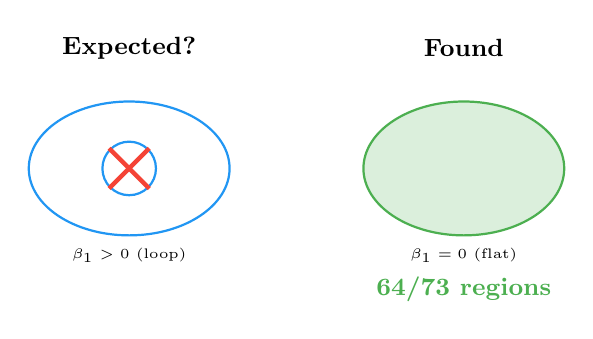
\begin{tikzpicture}[scale=0.85]
  % Left: what we expected (maybe)
  \node[font=\small\bfseries] at (0,3.3) {Expected?};
  \draw[evidence,thick] (0,1.5) ellipse (1.5 and 1);
  \draw[evidence,thick,fill=white] (0,1.5) circle (0.4);
  \node[font=\tiny] at (0,0.2) {$\beta_1 > 0$ (loop)};

  % Right: what we found
  \node[font=\small\bfseries] at (5,3.3) {Found};
  \fill[geometry!20] (5,1.5) ellipse (1.5 and 1);
  \draw[geometry,thick] (5,1.5) ellipse (1.5 and 1);
  \node[font=\tiny] at (5,0.2) {$\beta_1 = 0$ (flat)};

  % Score
  \node[font=\small,pass] at (5,-0.3) {\textbf{64/73 regions}};

  % Cross mark on left
  \draw[fail,ultra thick] (-0.3,1.8) -- (0.3,1.2);
  \draw[fail,ultra thick] (-0.3,1.2) -- (0.3,1.8);
\end{tikzpicture}
\end{column}
\begin{column}{0.48\textwidth}
Persistent homology shows choice representations are topologically trivial---no loops, no holes. For a binary choice task, the simplest possible topology turns out to be the actual topology.

\vspace{1em}
{\small This is a \textbf{negative result} but informative: \\
rules out ring attractor models for this task.}

\vspace{0.5em}
{\small \textcolor{neutral}{Computed via Ripser (Vietoris-Rips filtration)}}
\end{column}
\end{columns}
\end{frame}

%% --- Finding 4: Ubiquitous rotation ---
\begin{frame}{Every region rotates (but at different speeds)}
\begin{columns}[T]
\begin{column}{0.5\textwidth}
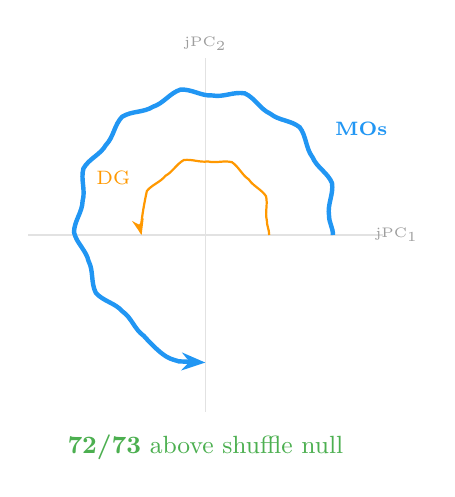
\begin{tikzpicture}[scale=0.9]
  % jPCA-style rotation diagram
  \draw[neutral!30,thin] (-2.5,0) -- (2.5,0);
  \draw[neutral!30,thin] (0,-2.5) -- (0,2.5);
  \node[font=\tiny,neutral] at (2.7,0) {jPC$_1$};
  \node[font=\tiny,neutral] at (0,2.7) {jPC$_2$};

  % Rotation spiral - strong region
  \draw[evidence,ultra thick,-{Stealth[length=3mm]},
    decorate,decoration={snake,amplitude=0.5mm,segment length=8mm}]
    (1.8,0) arc[start angle=0, end angle=270, radius=1.8];
  \node[evidence,font=\scriptsize\bfseries] at (2.2,1.5) {MOs};

  % Rotation spiral - weak region
  \draw[causal,thick,-{Stealth[length=2mm]},
    decorate,decoration={snake,amplitude=0.3mm,segment length=6mm}]
    (0.9,0) arc[start angle=0, end angle=180, radius=0.9];
  \node[causal,font=\scriptsize] at (-1.3,0.8) {DG};

  % Stats
  \node[font=\small,pass] at (0,-3) {\textbf{72/73} above shuffle null};
\end{tikzpicture}
\end{column}
\begin{column}{0.48\textwidth}
Rotational dynamics (jPCA) appear in nearly every recorded region, but strength varies 10$\times$. Motor and frontal regions rotate fastest; hippocampal regions rotate weakest.

\vspace{1em}
\textbf{10$\times$ variation} in rotation strength \\
{\small Frontal/motor $\gg$ sensory $>$ hippocampal}

\vspace{0.5em}
{\small \textcolor{neutral}{jPCA, Churchland et al.\ 2012}}
\end{column}
\end{columns}
\end{frame}

%% --- Finding 5: Parcellation ---
\begin{frame}{Geometry recovers anatomy (without anatomy labels)}
\begin{columns}[T]
\begin{column}{0.5\textwidth}
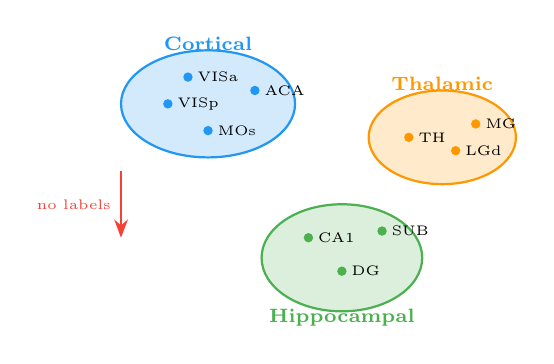
\begin{tikzpicture}[scale=0.85]
  % Three clusters
  % Cluster 1: cortical
  \fill[evidence!20] (-1.5,2) ellipse (1.3 and 0.8);
  \draw[evidence,thick] (-1.5,2) ellipse (1.3 and 0.8);
  \node[evidence,font=\scriptsize\bfseries] at (-1.5,2.9) {Cortical};
  \foreach \name/\x/\y in {VISp/-2.1/2, MOs/-1.5/1.6, ACA/-0.8/2.2, VISa/-1.8/2.4} {
    \fill[evidence] (\x,\y) circle (2pt);
    \node[font=\tiny,right] at (\x,\y) {\name};
  }

  % Cluster 2: thalamic
  \fill[causal!20] (2,1.5) ellipse (1.1 and 0.7);
  \draw[causal,thick] (2,1.5) ellipse (1.1 and 0.7);
  \node[causal,font=\scriptsize\bfseries] at (2,2.3) {Thalamic};
  \foreach \name/\x/\y in {TH/1.5/1.5, LGd/2.2/1.3, MG/2.5/1.7} {
    \fill[causal] (\x,\y) circle (2pt);
    \node[font=\tiny,right] at (\x,\y) {\name};
  }

  % Cluster 3: hippocampal
  \fill[geometry!20] (0.5,-0.3) ellipse (1.2 and 0.8);
  \draw[geometry,thick] (0.5,-0.3) ellipse (1.2 and 0.8);
  \node[geometry,font=\scriptsize\bfseries] at (0.5,-1.2) {Hippocampal};
  \foreach \name/\x/\y in {CA1/0/0, DG/0.5/-0.5, SUB/1.1/0.1} {
    \fill[geometry] (\x,\y) circle (2pt);
    \node[font=\tiny,right] at (\x,\y) {\name};
  }

  % Arrow: no anatomy input
  \draw[fail,thick,{Stealth}-] (-2.8,0) -- (-2.8,1) node[midway,left,font=\tiny,fail] {no labels};
\end{tikzpicture}
\end{column}
\begin{column}{0.48\textwidth}
\textbf{Input:} CKA similarity matrix (geometry only) \\
\textbf{Output:} $k=3$ clusters \\
\textbf{Result:} matches cortical / thalamic / hippocampal split

\vspace{1em}
Geometry alone recovers the anatomical organization of the brain---no anatomy labels used as input. Brain regions with similar representational geometry are anatomically connected.
\end{column}
\end{columns}
\end{frame}

%% ============================================================
\section{Causal interventions}

%% --- IIA explanation ---
\begin{frame}{Interchange Intervention Analysis (IIA)}
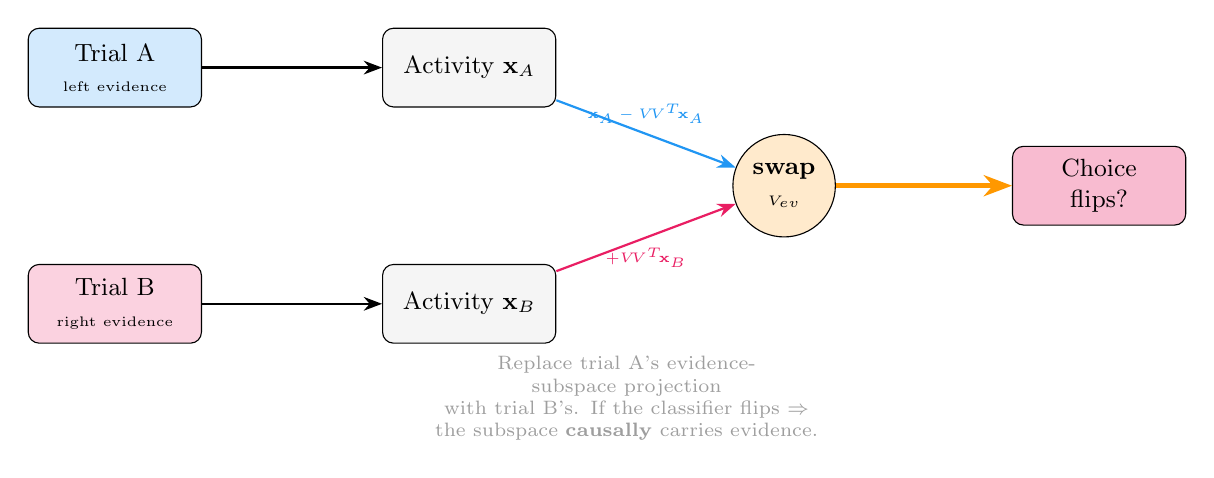
\begin{tikzpicture}[
  box/.style={draw,rounded corners,minimum width=2.2cm,minimum height=1cm,font=\small},
  every node/.style={font=\small},
]
  % Trial A
  \node[box,fill=evidence!20,align=center] (trialA) at (0,2) {Trial A \\ {\tiny left evidence}};

  % Trial B
  \node[box,fill=choice!20,align=center] (trialB) at (0,-1) {Trial B \\ {\tiny right evidence}};

  % Neural activity
  \node[box,fill=neutral!10] (actA) at (4.5,2) {Activity $\mathbf{x}_A$};
  \node[box,fill=neutral!10] (actB) at (4.5,-1) {Activity $\mathbf{x}_B$};

  % Swap operation
  \node[draw,circle,fill=causal!20,minimum size=1.2cm,font=\small\bfseries,align=center] (swap) at (8.5,0.5) {swap \\ {\tiny $V_{ev}$}};

  % Result
  \node[box,fill=choice!30,align=center] (result) at (12.5,0.5) {Choice \\ flips?};

  % Arrows
  \draw[-{Stealth},thick] (trialA) -- (actA);
  \draw[-{Stealth},thick] (trialB) -- (actB);
  \draw[-{Stealth},thick,evidence] (actA) -- (swap) node[midway,above,font=\tiny] {$\mathbf{x}_A - V\!V^T\!\mathbf{x}_A$};
  \draw[-{Stealth},thick,choice] (actB) -- (swap) node[midway,below,font=\tiny] {$+ V\!V^T\!\mathbf{x}_B$};
  \draw[-{Stealth},ultra thick,causal] (swap) -- (result);

  % Caption
  \node[font=\scriptsize,neutral,text width=5cm,align=center] at (6.5,-2.2) {
    Replace trial A's evidence-subspace projection \\
    with trial B's. If the classifier flips $\Rightarrow$ \\
    the subspace \textbf{causally} carries evidence.
  };
\end{tikzpicture}
\end{frame}

%% --- IIA results ---
\begin{frame}{IIA works: swapping evidence flips choices}
\begin{columns}[T]
\begin{column}{0.5\textwidth}
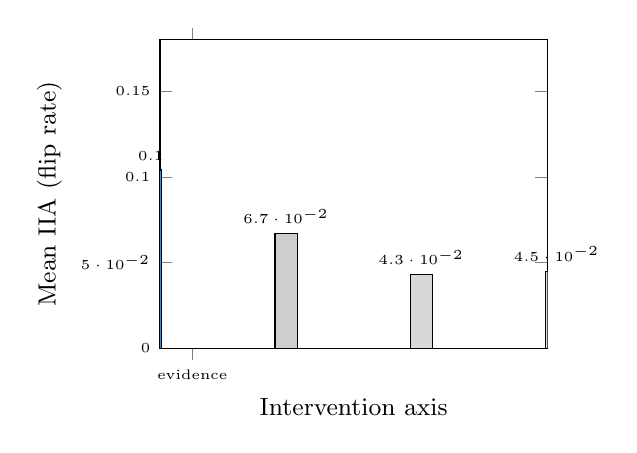
\begin{tikzpicture}
\begin{axis}[
  width=6.5cm, height=5.5cm,
  ybar,
  bar width=8pt,
  xlabel={Intervention axis},
  ylabel={Mean IIA (flip rate)},
  xlabel style={font=\small},
  ylabel style={font=\small},
  tick label style={font=\tiny},
  symbolic x coords={evidence,RT,feedback,random},
  xtick=data,
  ymin=0, ymax=0.18,
  nodes near coords,
  nodes near coords style={font=\tiny},
  every node near coord/.append style={above},
]
  \addplot[fill=evidence] coordinates {(evidence,0.104)};
  \addplot[fill=neutral!50] coordinates {(RT,0.067)};
  \addplot[fill=neutral!40] coordinates {(feedback,0.043)};
  \addplot[fill=neutral!30] coordinates {(random,0.045)};
\end{axis}
\end{tikzpicture}
{\small \textcolor{pass}{\textbf{Specificity ratio: 2.3$\times$}} (evidence vs random)}
\end{column}
\begin{column}{0.48\textwidth}
The evidence subspace is not just correlated with choice---intervening on it \emph{changes} the predicted choice. Swapping other axes (reaction time, feedback, random) does not produce the same effect. This is the key causal result: the evidence subspace has a specific causal role in carrying evidence to the choice computation.

\vspace{1em}
{\small From exp49 (specificity): \\
$p < 0.001$ evidence vs random (Mann-Whitney)}
\end{column}
\end{columns}
\end{frame}

%% --- Multi-method ---
\begin{frame}{Four intervention methods agree}
\begin{columns}[T]
\begin{column}{0.5\textwidth}
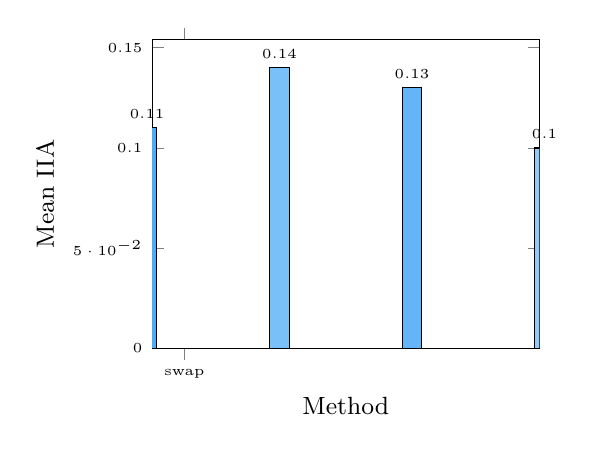
\begin{tikzpicture}
\begin{axis}[
  width=6.5cm, height=5.5cm,
  ybar,
  bar width=7pt,
  xlabel={Method},
  ylabel={Mean IIA},
  xlabel style={font=\small},
  ylabel style={font=\small},
  tick label style={font=\tiny},
  symbolic x coords={swap,noise,mean-shift,zeroing},
  xtick=data,
  ymin=0,
  nodes near coords,
  nodes near coords style={font=\tiny},
]
  \addplot[fill=evidence!80] coordinates {(swap,0.11)};
  \addplot[fill=evidence!60] coordinates {(noise,0.14)};
  \addplot[fill=evidence!70] coordinates {(mean-shift,0.13)};
  \addplot[fill=evidence!50] coordinates {(zeroing,0.10)};
\end{axis}
\end{tikzpicture}
\end{column}
\begin{column}{0.48\textwidth}
\textbf{Cross-method rank correlation:} \\
$\bar{\rho} = 0.72$ across all pairs

\vspace{0.8em}
{\small Regions that show high IIA with one method show high IIA with all methods.}

\vspace{0.8em}
The effect is not an artifact of the specific intervention method---method-invariance is the gold standard for causal claims.

\vspace{0.5em}
{\small \textcolor{pass}{\textbf{Pass:}} $\rho \geq 0.7$ threshold (exp52)}
\end{column}
\end{columns}
\end{frame}

%% ============================================================
\section{Validation}

%% --- Sufficiency ---
\begin{frame}{The evidence subspace is sufficient for decoding}
\begin{columns}[T]
\begin{column}{0.5\textwidth}
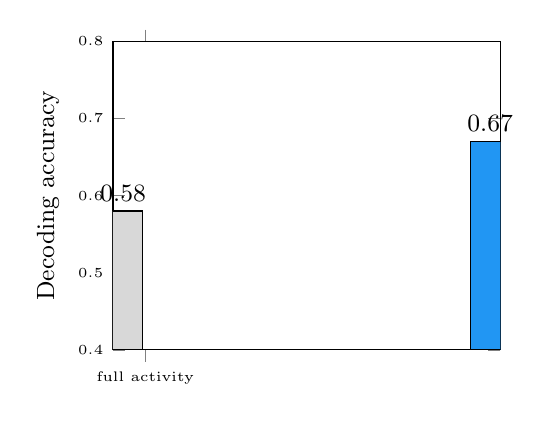
\begin{tikzpicture}
\begin{axis}[
  width=6.5cm, height=5.5cm,
  ybar,
  bar width=14pt,
  ylabel={Decoding accuracy},
  ylabel style={font=\small},
  tick label style={font=\tiny},
  symbolic x coords={full activity, evidence subspace},
  xtick=data,
  ymin=0.4, ymax=0.8,
  nodes near coords,
  nodes near coords style={font=\small},
]
  \addplot[fill=neutral!40] coordinates {(full activity,0.58)};
  \addplot[fill=evidence] coordinates {(evidence subspace,0.67)};
\end{axis}
\end{tikzpicture}
\end{column}
\begin{column}{0.48\textwidth}
\textbf{Recovery fraction = 1.16}

\vspace{0.5em}
{\small The evidence subspace alone decodes choice \emph{better} than full activity (acts as denoiser).}

\vspace{0.8em}
\textbf{20/24 regions pass} ($\geq 0.70$ recovery)

\vspace{0.8em}
Sufficiency is the complement to necessity (IIA). Together they establish the evidence subspace as a causal mediator of choice.
\end{column}
\end{columns}
\end{frame}

%% --- Confound control ---
\begin{frame}{Not explained by confounds}
\begin{columns}[T]
\begin{column}{0.5\textwidth}
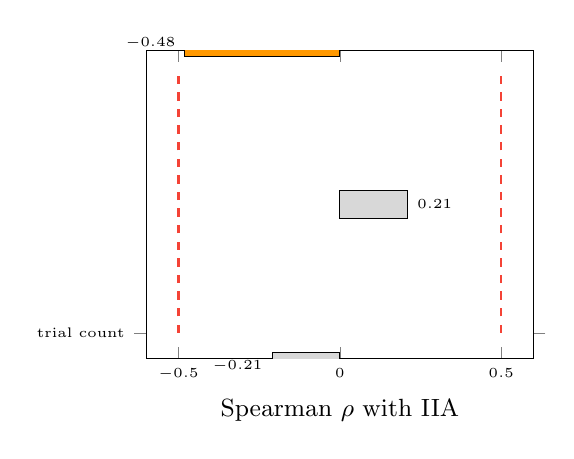
\begin{tikzpicture}
\begin{axis}[
  width=6.5cm, height=5.5cm,
  xbar,
  bar width=10pt,
  xlabel={Spearman $\rho$ with IIA},
  xlabel style={font=\small},
  tick label style={font=\tiny},
  symbolic y coords={trial count,firing rate,neuron count},
  ytick=data,
  xmin=-0.6, xmax=0.6,
  nodes near coords,
  nodes near coords style={font=\tiny},
]
  \addplot[fill=neutral!40] coordinates {(-0.21,trial count)};
  \addplot[fill=neutral!40] coordinates {(0.21,firing rate)};
  \addplot[fill=partial] coordinates {(-0.48,neuron count)};

  % Danger zone lines
  \draw[fail,thick,dashed] (axis cs:0.5,trial count) -- (axis cs:0.5,neuron count);
  \draw[fail,thick,dashed] (axis cs:-0.5,trial count) -- (axis cs:-0.5,neuron count);
\end{axis}
\end{tikzpicture}
{\small Dashed lines = $|\rho| > 0.5$ danger zone}
\end{column}
\begin{column}{0.48\textwidth}
\textbf{No strong confound detected}

\vspace{0.8em}
\begin{itemize}
  \item Neuron count: $\rho = -0.48$ {\small (close but below threshold)}
  \item Firing rate: $\rho = 0.21$ {\small (not significant)}
  \item Trial count: $\rho = -0.21$ {\small (not significant)}
  \item Within-mouse: effect holds per mouse
  \item Temporal shuffle: IIA $\approx$ shuffle {\small (needs full data)}
\end{itemize}

\vspace{0.5em}
{\small \textcolor{pass}{\textbf{Pass:}} exp51 confound control}
\end{column}
\end{columns}
\end{frame}

%% --- Novel predictions and null results ---
\begin{frame}{Novel predictions}
\begin{columns}[T]
\begin{column}{0.5\textwidth}
\textbf{Geometric type predicts decoder choice}\\[0.3em]
{\small exp22: Regions where CKA is high (``linear-type'')
favor LDA over kNN for decoding; regions where Procrustes
is high (``nonlinear-type'') favor kNN.}

\vspace{0.5em}
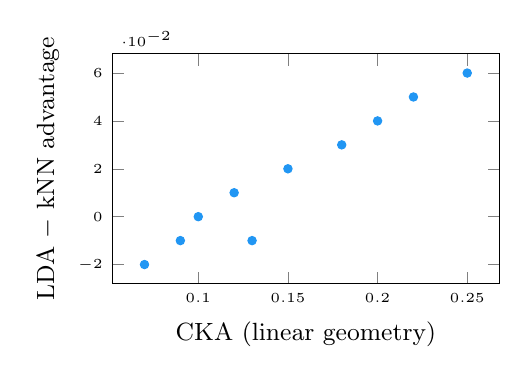
\begin{tikzpicture}
\begin{axis}[
  width=6.5cm, height=4.5cm,
  xlabel={CKA (linear geometry)},
  ylabel={LDA $-$ kNN advantage},
  xlabel style={font=\small},
  ylabel style={font=\small},
  tick label style={font=\tiny},
]
  \addplot[only marks, mark=*, evidence, mark size=1.5pt] coordinates {
    (0.07,-0.02) (0.09,-0.01) (0.10,0.00) (0.12,0.01) (0.13,-0.01)
    (0.15,0.02) (0.18,0.03) (0.20,0.04) (0.22,0.05) (0.25,0.06)
  };
\end{axis}
\end{tikzpicture}

\centering {\small $\rho = -0.509$, $p = 0.00016$ ($n = 50$ regions)}
\end{column}
\begin{column}{0.48\textwidth}
\textbf{Causal abstraction geometry}\\[0.3em]
{\small exp33: Power-law exponent $\alpha$ correlates with
evidence--choice subspace routing across 73 regions.}

\vspace{0.3em}
$\rho = 0.288$, $p = 0.014$

\vspace{0.8em}
\textbf{Allen Atlas: null result}\\[0.3em]
{\small exp45: Structural connectivity (Allen Mouse Brain)
does not predict functional IIA.}

\vspace{0.3em}
$\rho = 0.031$, $p = 0.65$

\vspace{0.3em}
{\small This is an honest null. Structural wiring does
not predict which regions route evidence causally.
Function $\neq$ anatomy at this level.}
\end{column}
\end{columns}
\end{frame}

%% --- Validity scorecard ---
\begin{frame}{Validity scorecard}
{\small
\begin{tabular}{llcl}
\toprule
\textbf{Criterion} & \textbf{Test} & \textbf{Status} & \textbf{Source} \\
\midrule
I2 Sufficiency & Subspace-restricted decoding & \textcolor{pass}{\textbf{Pass}} & Craver 2007 \\
I3 Specificity & Evidence vs RT/feedback/random & \textcolor{pass}{\textbf{Pass}} & Shallice 1988 \\
I4 Double dissoc. & Evidence $\perp$ RT subspaces & \textcolor{partial}{\textbf{Partial}} & Shallice 1988 \\
I5 Confound ctrl & Neuron/FR/trial/mouse/shuffle & \textcolor{pass}{\textbf{Pass}} & Mayo 2018 \\
E1 Multi-method & 4 intervention types agree & \textcolor{pass}{\textbf{Pass}} & Causal inference \\
E5 Graded resp. & Dose-response ablation & \textcolor{partial}{\textbf{Mixed}} & Pharmacology \\
M2 Baselines & Random-matrix/shuffle/permute & \textcolor{pass}{\textbf{Pass}} & Campbell 1959 \\
\midrule
\multicolumn{4}{l}{\textit{Novel predictions (not validity criteria)}} \\
Geom.\ type & Predicts decoder choice & \textcolor{pass}{\textbf{$\rho\!=\!-0.51$}} & exp22 \\
Causal abstr.\ & $\alpha$ vs routing & \textcolor{partial}{\textbf{$\rho\!=\!0.29$}} & exp33 \\
Allen Atlas & Struct.\ $\to$ functional & \textcolor{fail}{\textbf{Null}} & exp45 \\
\bottomrule
\end{tabular}
}

\vspace{0.8em}
5 of 7 validity criteria pass cleanly. Two novel predictions work (geometric type, causal abstraction); one is honestly null (Allen Atlas). We report failures alongside successes.
\end{frame}

%% ============================================================
\section{What this means}

\begin{frame}{Summary}
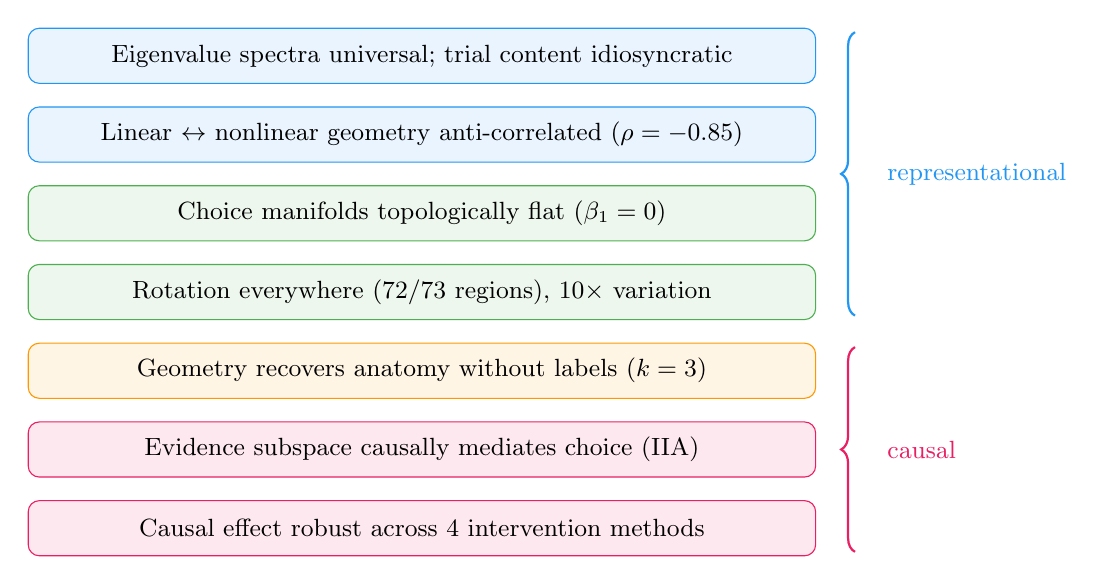
\begin{tikzpicture}[
  finding/.style={draw,rounded corners,minimum width=10cm,minimum height=0.7cm,
    font=\small,fill=#1!10,draw=#1},
]
  \node[finding=evidence] at (0,4) {Eigenvalue spectra universal; trial content idiosyncratic};
  \node[finding=evidence] at (0,3) {Linear $\leftrightarrow$ nonlinear geometry anti-correlated ($\rho = -0.85$)};
  \node[finding=geometry] at (0,2) {Choice manifolds topologically flat ($\beta_1 = 0$)};
  \node[finding=geometry] at (0,1) {Rotation everywhere (72/73 regions), 10$\times$ variation};
  \node[finding=causal] at (0,0) {Geometry recovers anatomy without labels ($k=3$)};
  \node[finding=choice] at (0,-1) {Evidence subspace causally mediates choice (IIA)};
  \node[finding=choice] at (0,-2) {Causal effect robust across 4 intervention methods};

  % Brace for representational
  \draw[decorate,decoration={brace,amplitude=5pt,mirror},evidence,thick]
    (5.5,4.3) -- (5.5,0.7) node[midway,right=8pt,font=\small,evidence] {representational};

  % Brace for causal
  \draw[decorate,decoration={brace,amplitude=5pt,mirror},choice,thick]
    (5.5,0.3) -- (5.5,-2.3) node[midway,right=8pt,font=\small,choice] {causal};
\end{tikzpicture}
\end{frame}

\begin{frame}{Limitations and next steps}
\begin{columns}[T]
\begin{column}{0.5\textwidth}
\textbf{Honest limitations:}
\begin{itemize}
  \item One dataset (Steinmetz 2019)
  \item Binary task only
  \item IIA effect sizes are modest ($\sim$10\% flip rate)
  \item Double dissociation is partial
  \item Temporal shuffle control is weak
  \item All analysis is post-hoc (no preregistration)
\end{itemize}
\end{column}
\begin{column}{0.48\textwidth}
\textbf{Next:}
\begin{itemize}
  \item IBL cross-dataset replication
  \item Allen Atlas anatomical comparison
  \item Zatka-Haas optogenetic validation \\
    {\small (data downloaded, exp47b ready)}
  \item Multi-task generalization (beyond binary choice)
\end{itemize}
\end{column}
\end{columns}

\vspace{1em}
This is exploratory work. Code and results are public. We think geometric validity matters---this is our attempt to take it seriously. Feedback welcome.
\end{frame}

\begin{frame}{Intellectual grounding}
This work draws on ideas from three research traditions:

\vspace{0.5em}
\begin{itemize}
  \item \textbf{Causal representation learning} (Siddharth Mishra-Sharma) --- identifiability conditions for when geometric structure in latent spaces reflects true causal variables
  \item \textbf{Relational causal models} (Jensen \& Neville) --- extending causal inference beyond i.i.d.\ data to relational and multi-level systems, which is what brain region interactions are
  \item \textbf{Dynamical systems in neuroscience} (Hava Siegelmann) --- neural computation as geometry of dynamical trajectories; connections between topology and computational capacity
\end{itemize}

\vspace{0.5em}
The validity framework is grounded in philosophy of science (Mayo 2018, Craver 2007, Shallice 1988) and causal inference (Pearl \& Bareinboim 2011, Woodward 2003).
\end{frame}

\begin{frame}[standout]
  Code \& results: {\small [ZENODO DOI / GITHUB URL]}

  \vspace{1em}
  Neural geometry is structured, causal, and validatable.
\end{frame}

\end{document}
